\documentclass[../main.tex]{subfiles}
\graphicspath{{\subfix{../Figures/}}}
\begin{document}
	\begin{frame}{Experiments}
		We performed some experiments to show empirically our mixing result. 
		\begin{itemize}
			\item First, we want to prove that the mixing time grows logarithmically with the volume, and decreases quadratically with the conductance, namely $t=O\left(\frac{\log(n)}{\hat{\phi}^2}\right).$
			\item We know that for $r$-uniform hypergraphs there is a theoretical upper-bound for the continuous diffusion process $t=O\left(\frac{\log(n)}{\hat{\phi}^2 r}\right)$. We want to see if such upper bound also holds for our simplified discrete diffusion process.
		\end{itemize}
	\end{frame}

	\begin{frame}{Experiment 1}
		\begin{columns}
		\column{0.5\textwidth}
		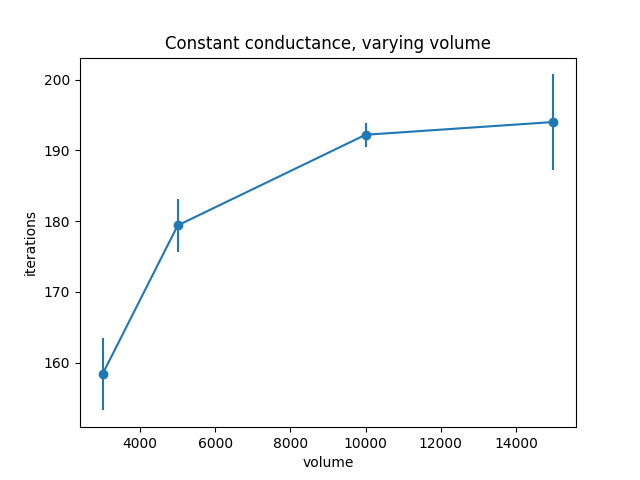
\includegraphics[width=0.9\textwidth]{Figures/const_cond}  
		\column{0.4\textwidth}
		When the conductance is constant and the volume changes, the mixing time is \textit{logarithmic} wrt the volume. 
		\end{columns} 
		\begin{columns}
			\column{0.5\textwidth}
			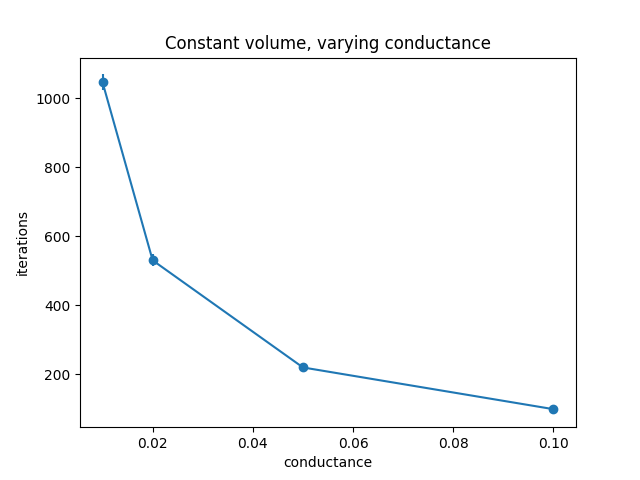
\includegraphics[width=0.9\textwidth]{Figures/const_vol}  
			\column{0.4\textwidth}
			Instead, when the volume is constant and the conductance changes, then the mixing time decreases \textit{quadratically} fast.
		\end{columns} 
	\end{frame}

	\begin{frame}{Experiment 2}
		\begin{columns}
			\column{0.6\textwidth}
			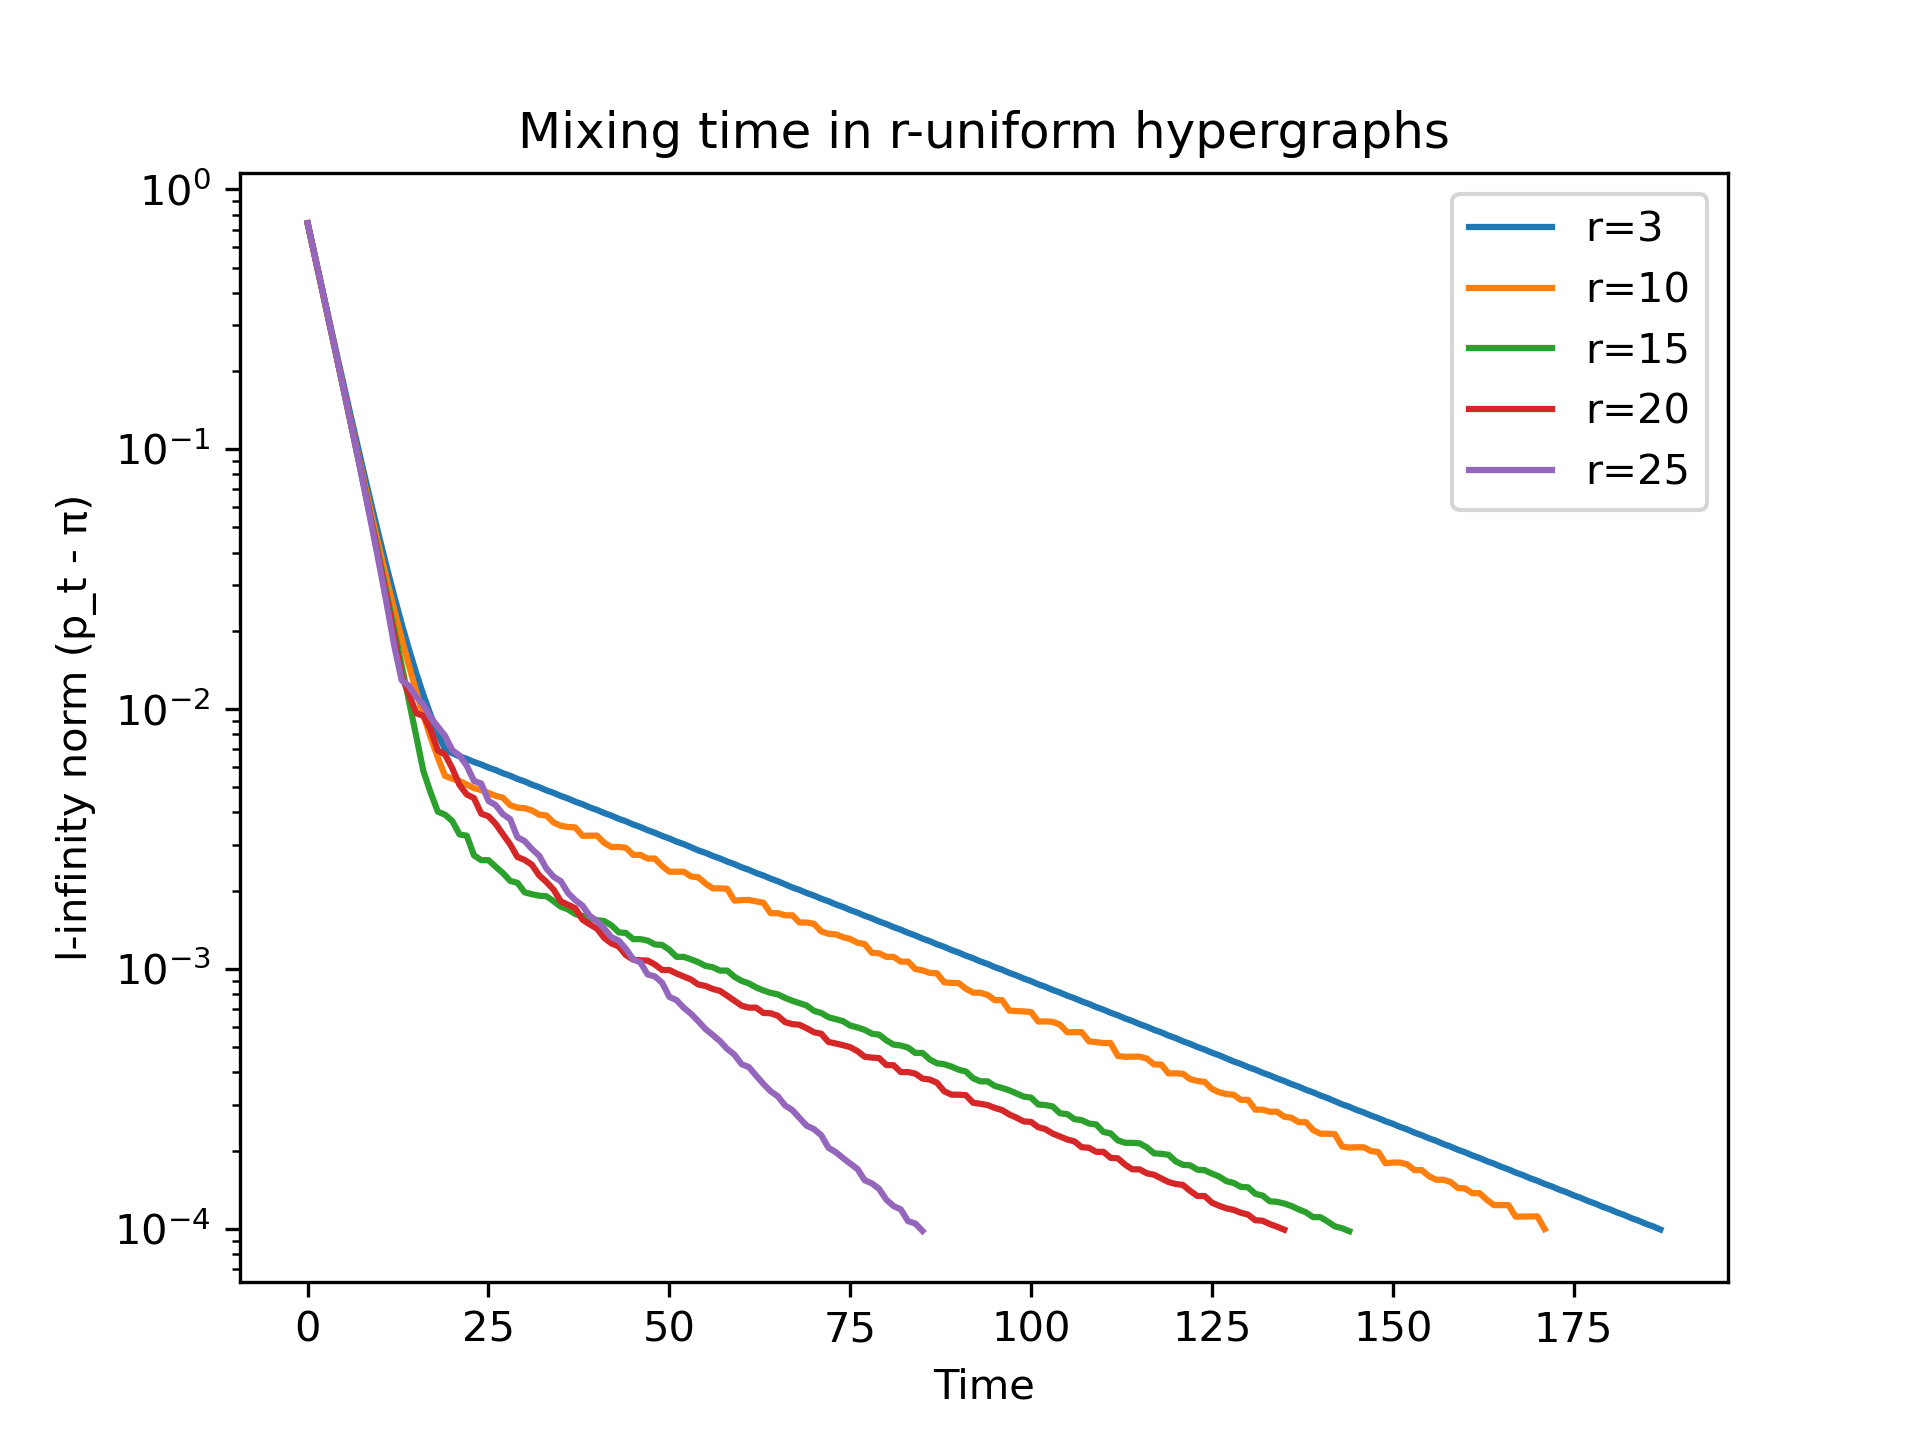
\includegraphics[width=1\textwidth]{Figures/mixing_r_uniform_hypergraph}  
			\column{0.4\textwidth}
			Indeed, the larger the $r$ the smaller the mixing time, suggesting that also with our discrete diffusion process when the hypergraph is $r$-uniform it might hold $t=O\left(\frac{\log(n)}{r\hat{\phi}^2}\right)$.
		\end{columns}
	\end{frame}
\end{document}